\documentclass{beamer}
\usetheme{CambridgeUS}
\usecolortheme{dolphin}
\usepackage{tikz}

\usepackage{tcolorbox}
\usetikzlibrary{shapes.geometric, arrows, positioning,spy,fit,backgrounds,arrows.meta}
\usepackage{pgfplots}
\usepackage{listings}
\usepackage{xcolor}
\lstset{
    basicstyle=\ttfamily\scriptsize,
    keywordstyle=\color{blue}\bfseries,
    commentstyle=\color{green!60!black},
    stringstyle=\color{red},
    showstringspaces=false,
    frame=single,
    breaklines=true,
    captionpos=b
}

\usetikzlibrary{shapes.geometric, arrows, positioning,spy,fit,backgrounds,arrows.meta}
\usepackage{pgfplots}
\usepackage{fontawesome5}
\pgfplotsset{compat=1.17}

\useinnertheme{rectangles}
\useoutertheme{miniframes}

% Add this in the preamble
\setbeamertemplate{footline}{
    \leavevmode%
    \hbox{%
        \begin{beamercolorbox}[wd=.5\paperwidth,ht=2.25ex,dp=1ex,left]{date in head/foot}%
            \hspace*{2ex}\usebeamerfont{date in head/foot}\insertdate
        \end{beamercolorbox}%
        \begin{beamercolorbox}[wd=.5\paperwidth,ht=2.25ex,dp=1ex,right]{date in head/foot}%
            \usebeamerfont{date in head/foot}\insertframenumber{} / \inserttotalframenumber\hspace*{2ex}
        \end{beamercolorbox}}%
    \vskip0pt%
}

% Remove navigation symbols
\setbeamertemplate{navigation symbols}{}

\setbeamercolor*{mini frame}{fg=black,bg=white}
\setbeamercolor{section in head/foot}{fg=black, bg=white}

\definecolor{myred}{RGB}{204, 51, 51} % Define mild moderate red
\definecolor{lightgray}{RGB}{240, 240, 240} % Light gray for block background

\setbeamercolor{structure}{fg=myred} % Color of text elements
\setbeamercolor{alerted text}{fg=red} % Color of alerted text (e.g., \alert{})
\setbeamercolor{block title}{bg=myred,fg=white} % Color of block titles
\setbeamercolor{block body}{bg=lightgray} % Color of block body
\setbeamercolor{block title alerted}{bg=myred,fg=white} % Color of block titles
\setbeamercolor{block body alerted}{bg=lightgray} % Color of block body
\setbeamercolor{itemize item}{fg=myred} % Color of itemize bullets
\setbeamercolor{itemize subitem}{fg=myred} % Color of sub-itemize bullets
\setbeamercolor{enumerate item}{fg=myred} % Color of enumerate bullets
\setbeamercolor{enumerate subitem}{fg=myred} % Color of sub-enumerate bullets
\setbeamercolor{title}{fg=myred} % Color of title
\setbeamercolor{author}{fg=black} % Color of author
\setbeamercolor{date}{fg=black} % Color of date

% Define TikZ styles
\tikzstyle{startstop} = [rectangle,rounded corners, minimum width=1.5cm, minimum height=1cm, text centered,align=center, draw=black, fill=red!30]
\tikzstyle{process} = [rectangle,rounded corners, minimum width=1.5cm, minimum height=1cm, text centered, draw=black,align=center, fill=orange!30]
\tikzstyle{midprocess} = [rectangle,rounded corners, minimum width=1.5cm, minimum height=1cm, text centered, draw=black,align=center, fill=myred!30]
\tikzstyle{decision} = [diamond, minimum width=1.5cm, minimum height=1cm, text centered, draw=black,align=center, fill=myred!30]
\tikzstyle{arrow} = [thick,->,>=stealth]

\AtBeginSection[]{
    \begin{frame}
        \tableofcontents[currentsection, hideothersubsections]
    \end{frame}
}


\title{EasyJailbreak: A Unified Framework for Jailbreaking Large Language
Models}

% Author details
\author{
    \textbf{\large Authored by:} \\ \vspace{0.3cm}
    Weikang Zhou \and
    Xiao Wang \and
    Limao Xiong \and
    Han Xia \and
    Yingshuang Gu \and
    Mingxu Chai \and
    Fukang Zhu \and
    Caishuang Huang \and
    Tao Gui \and
    Qi Zhang \and
    Xuanjing Huang \\ \vspace{0.3cm}
    \textbf{\large Presented by:} \\ \vspace{0.3cm}
    Himadri Gobinda Biswas-2105047\\ \and Shams Hossain Simanto-2105048\\ \and Nawriz Ahmed Turjo-2105032
}

\date{December 8, 2024}

\begin{document}

\frame{\titlepage}

% \begin{frame}
%     \centering
%     A Simple Thought Experiment
% \end{frame}

\begin{frame}
    \tableofcontents[sectionstyle=show,subsectionstyle=show/shaded/hide,subsubsectionstyle=show/shaded/hide]
\end{frame}



\section{Introduction}
\begin{frame}{Introduction to Jailbreaking}

  \begin{block}{What is jailbreaking?} \pause
    \textit{A method to bypass safeguards in Large Language Models (LLMs) to elicit prohibited or unintended outputs.}
  \end{block}
\end{frame}

\begin{frame}{Introduction to Jailbreaking}
    \begin{figure}[h]
    \centering
    \includegraphics[scale=0.45,width=0.8\textwidth]{pic/JailBreakingDef.jpg}
    \label{fig:enter-label2}
    \end{figure}
\end{frame}



\begin{frame}{Jailbreaking as a research topic}
    \centering
    \begin{tikzpicture}[node distance=2.2cm]

        % Define TikZ styles
        \tikzstyle{centerblock} = [circle, minimum width=1.8cm, minimum height=1.8cm, text centered, draw=black, fill=red!80, text=white]
        \tikzstyle{block} = [rectangle, rounded corners, minimum width=2.5cm, minimum height=1cm, text centered, draw=white, fill=blue!60, text=white]
        \tikzstyle{arrow} = [thick,->,>=stealth]

        % Central Node
        \onslide<1->{\node (challenges) [centerblock] {Objectives};}

        % Upper Left Node
        \onslide<2->{\node(shortage)[above left of=challenges, xshift=-1.2cm, yshift=0.8cm]{\includegraphics[width=0.8cm]{stickers/identify.png}};}
        \onslide<2->{\node (shortagetext) [above left of=challenges, xshift=-1.2cm, yshift=0.1cm] {\tiny Identify vulnerabilities in LLMs};}
        \onslide<2->{\node[draw, thick, rounded corners, fit=(shortage)(shortagetext)] {}; }

        % Upper Right Node
        \onslide<3->{\node(images)[above right of=challenges, xshift=1.2cm, yshift=0.8cm]{\includegraphics[width=0.8cm]{stickers/shield.png}};}
        \onslide<3->{\node (imagestext) [above right of=challenges, xshift=1.2cm, yshift=0.1cm] {\tiny Improve model safety and robustness};}
        \onslide<3->{\node[draw, thick, rounded corners, fit=(images)(imagestext)] {}; }

        % Lower Left Node
        \onslide<4->{\node(reports)[below left of=challenges, xshift=-1.2cm, yshift=-0.8cm]{\includegraphics[width=0.8cm]{stickers/Malicious_use.png}};}
        \onslide<4->{\node (reportstext) [below left of=challenges, xshift=-1.2cm, yshift=-1.5cm] {\tiny Test defenses against malicious use};}
        \onslide<4->{\node[draw, thick, rounded corners, fit=(reports)(reportstext)] {}; }

        % Lower Right Node
        \onslide<5->{\node(protocols)[below right of=challenges, xshift=1.2cm, yshift=-0.8cm]{\includegraphics[width=0.8cm]{stickers/security-protocol.png}};}
        \onslide<5->{\node (protocolstext) [below right of=challenges, xshift=1.2cm, yshift=-1.5cm] {\tiny Develop better security protocols};}
        \onslide<5->{\node[draw, thick, rounded corners, fit=(protocols)(protocolstext)] {}; }

    \end{tikzpicture}
\end{frame}


\section{Related Work}


\begin{frame}{Related Work}
    % Introductory Line
    \onslide<1->{\centering Current jailbreaking methodologies fall into 3 categories.}

    \vspace{0.8cm} % Reduced space between the line and the TikZ diagram

    \begin{tikzpicture}[node distance=1.8cm] % Reduced overall node distance

        % Define TikZ styles
        \tikzstyle{centerblock} = [circle, minimum width=1.5cm, minimum height=1.5cm, text centered, draw=black, fill=red!80, text=white, align=center]
        \tikzstyle{block} = [rectangle, rounded corners, minimum width=2.5cm, minimum height=0.8cm, text centered, draw=white, fill=blue!60, text=white]
        \tikzstyle{arrow} = [thick,->,>=stealth]

        % Central Node (with two-line text)
        \onslide<1->{\node (current_methods) [centerblock] {Current \\ Methods};}

        % Upper Left Node
        \onslide<2->{\node (human_design_icon) [above left of=current_methods, xshift=-1cm, yshift=0.6cm] {\includegraphics[width=0.8cm]{stickers/coding.png}};}
        \onslide<2->{\node (human_design_text) [above left of=current_methods, xshift=-1cm, yshift=0cm] {Human Design};}
        \onslide<2->{\node[draw, thick, rounded corners, fit=(human_design_icon)(human_design_text)] {};}

        % Upper Right Node
        \onslide<3->{\node (long_tail_icon) [above right of=current_methods, xshift=1.3cm, yshift=0.6cm] {\includegraphics[width=0.8cm]{stickers/encode.png}};}
        \onslide<3->{\node (long_tail_text) [above right of=current_methods, xshift=1.3cm, yshift=0cm] {Long-tail Encoding};}
        \onslide<3->{\node[draw, thick, rounded corners, fit=(long_tail_icon)(long_tail_text)] {};}

        % Below Node
        \onslide<4->{\node (prompt_opt_icon) [below of=current_methods, yshift=-0.4cm] {\includegraphics[width=0.8cm]{stickers/speed-radar.png}};}
        \onslide<4->{\node (prompt_opt_text) [below of=current_methods, yshift=-0.9cm] {Prompt Optimization};}
        \onslide<4->{\node[draw, thick, rounded corners, fit=(prompt_opt_icon)(prompt_opt_text)] {};}

    \end{tikzpicture}
\end{frame}




% \section{Limitations of Existing Approaches}
\begin{frame}{Limitations of Existing Approaches} \pause
    \begin{itemize}
        \item Fair comparison is hard due to varying datasets and models. \pause
        \item Lack of source code makes reproducing prior work slow and error-prone. \pause
        \item  These barriers complicate identifying and addressing LLM vulnerabilities. 
    \end{itemize}
\end{frame}



\begin{frame}{Features of EasyJailbreak}
    \onslide<1->{
        \centering
        EasyJailbreak addresses these limitations by offering the following features:
    }
    \vspace{0.5cm}
    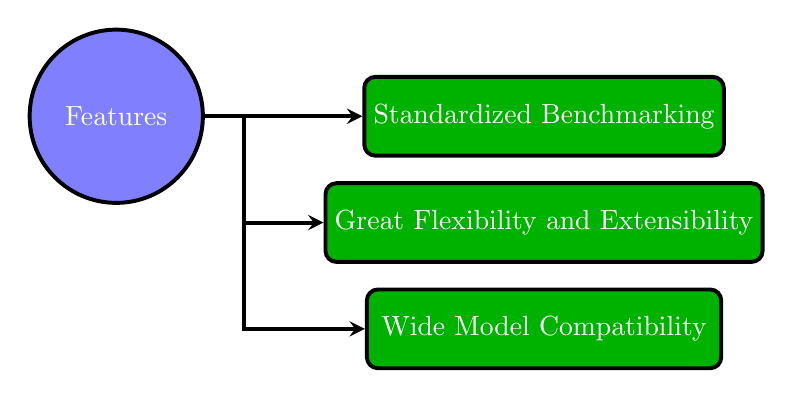
\begin{tikzpicture}[node distance=1.5cm and 2cm, >=stealth, thick]

        % Circle in the center-left (Smaller radius)
        \onslide<1->{\node[circle, draw=black, fill=blue!50, text=white, minimum size=2.2cm, text centered, line width=0.5mm,yshift=-1.5cm] (features) {Features};}

        % Horizontal blocks (Darker green rectangles)
        \onslide<2->{\node[rectangle, rounded corners, draw=black, fill=green!70!black, text=white, minimum width=4.5cm, minimum height=1cm, right=of features, line width=0.5mm] (benchmarking) {Standardized Benchmarking};}
        \onslide<3->{\node[rectangle, rounded corners, draw=black, fill=green!70!black, text=white, minimum width=4.5cm, minimum height=1cm, below=0.3cm of benchmarking, line width=0.5mm] (flexibility) {Great Flexibility and Extensibility};}
        \onslide<4->{\node[rectangle, rounded corners, draw=black, fill=green!70!black, text=white, minimum width=4.5cm, minimum height=1cm, below=0.3cm of flexibility, line width=0.5mm] (compatibility) {Wide Model Compatibility};}

        % Black arrows connecting the circle to each block
        \onslide<2->{\draw[->, line width=0.5mm, black] (features.east) -- ++(0.5cm,0) |- (benchmarking.west);}
        \onslide<3->{\draw[->, line width=0.5mm, black] (features.east) -- ++(0.5cm,0) |- (flexibility.west);}
        \onslide<4->{\draw[->, line width=0.5mm, black] (features.east) -- ++(0.5cm,0) |- (compatibility.west);}

    \end{tikzpicture}
\end{frame}


\section{Framework}
\begin{frame}{Framework diagram}

    \begin{figure}[h]
    \centering
    %\includegraphics[scale=0.3,width=0.8\textwidth]{pic/FrameworkDg3.jpg}
    \includegraphics[scale=0.3,width=0.9\textwidth]{pic/FrameworkDg3.jpg}
    %\caption{The farmework of \textit{EasyJailbreak}}
    \label{fig:enter-label21}
    \end{figure}

\end{frame}

% -------------------------------------------------------Simanto


\begin{frame}{Steps To Conduct A Jailbreak Attack}
    \centering
    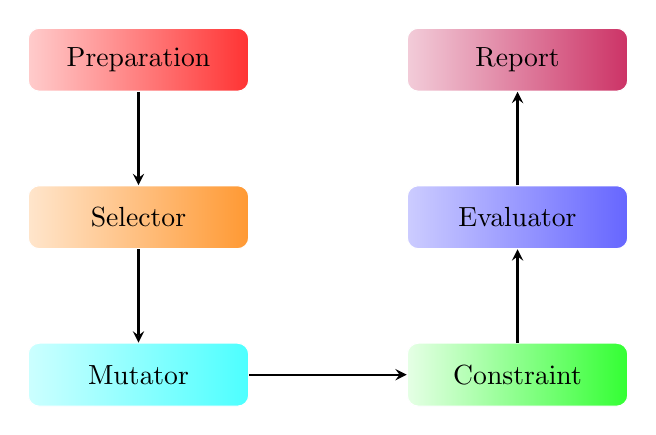
\begin{tikzpicture}[
        node distance=2cm, % Spacing between nodes
        arrow/.style={thick, ->, >=stealth}, % Arrow style
        every node/.style={rectangle, rounded corners, draw=white, fill=blue!20, minimum height=0.8cm, minimum width=2.8cm, text centered} % Node style
    ]

        % Left vertical flow (downward)
        \node (prep) [shading=axis, left color=red!20, right color=red!80] {Preparation};
        \node (selector) [below of=prep, shading=axis, left color=orange!20, right color=orange!80] {Selector};
        \node (mutator) [below of=selector, shading=axis, left color=cyan!20, right color=cyan!70] {Mutator};

        % Bottom horizontal flow (rightward)
        \node (constraint) [right=2cm of mutator, shading=axis, left color=green!10, right color=green!80] {Constraint};

        % Right vertical flow (upward)
        \node (evaluator) [above of=constraint, shading=axis, left color=blue!20, right color=blue!60] {Evaluator};
        \node (report) [above of=evaluator, shading=axis, left color=purple!20, right color=purple!80] {Report};

        % Connect the left vertical flow
        \draw [arrow] (prep) -- (selector);
        \draw [arrow] (selector) -- (mutator);

        % Connect the bottom horizontal flow
        \draw [arrow] (mutator) -- (constraint);

        % Connect the right vertical flow
        \draw [arrow] (constraint) -- (evaluator);
        \draw [arrow] (evaluator) -- (report);

    \end{tikzpicture}
\end{frame}

\begin{frame}{Preparation}
    % Add a question box at the top
    % \vspace{1cm}
    \begin{tikzpicture}[remember picture, overlay]
        \node[rectangle, draw=blue!70, fill=blue!10, rounded corners, text width=0.9\textwidth, % Wider block
              text centered, inner sep=5pt, % Smaller vertical padding
              anchor=north, shading=axis, left color=blue!10, right color=blue!40] 
              (questionblock) at ([yshift=-2cm]current page.north) {
            \includegraphics[width=1cm]{stickers/question.png} \hspace{0.2cm}
            \textbf{What do we even do in the preparation phase?}
        };
    \end{tikzpicture}
    \pause
    \vspace{1cm} % Adjust spacing below the question box

    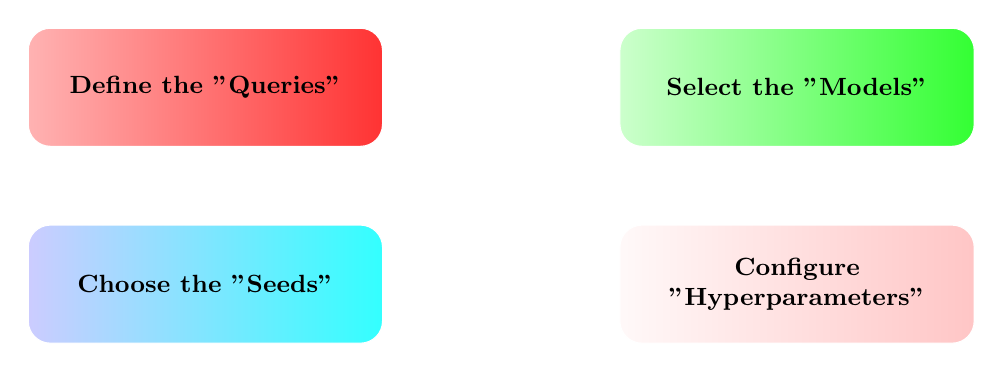
\begin{tikzpicture}[
        node distance=1.5cm, 
        every node/.style={
            rectangle, 
            draw=white, % Thicker black border
            rounded corners=8pt, % Smooth rounded corners
            minimum width=4.5cm, 
            minimum height=1.5cm, % Balanced height
            text width=4cm, 
            align=center,
            shading=axis, % Add gradient shading
            font=\bfseries\small % Bold and smaller font for modern look
            % drop shadow={fill=black, opacity=0.15, blur radius=5pt} % Shadow effect
        }
    ]
        % Left side nodes
        \node (queries) [left color=red!30, right color=red!80] {Define the "Queries"};\pause
        \node (seeds) [below of=queries, yshift=-1cm, left color=blue!20, right color=cyan!80] {Choose the "Seeds"};\pause

        % Right side nodes
        \node (models) [right=3cm of queries, left color=green!20, right color=green!80] {Select the "Models"};\pause
        \node (hyperparams) [right=3cm of seeds, left color=pink!10, right color=pink!90] {Configure \\"Hyperparameters"};

    \end{tikzpicture}
\end{frame}



\begin{frame}{Understanding the Key Terms}
    % Smaller Question Block at the Top
    \begin{tikzpicture}[remember picture, overlay]
        \node[rectangle, draw=blue!70, fill=blue!10, rounded corners, text width=0.7\textwidth, 
              text centered, inner sep=5pt, anchor=north, shading=axis, left color=blue!10, right color=blue!40] 
              (questionblock) at ([yshift=-3cm]current page.north) {
            \includegraphics[width=1cm]{stickers/question.png} \hspace{0.2cm}
            \textbf{What are queries, seeds, models, and hyperparameters?}
        };
    \end{tikzpicture}\pause

    \vspace{2cm}
    % Explanation Block Centered
    \begin{tikzpicture}[remember picture, overlay]
        \node[rectangle, draw=cyan!70, fill=cyan!10, rounded corners, text width=0.6\textwidth, 
              text centered, inner sep=10pt, shading=axis, left color=cyan!10, right color=cyan!50] 
              (exampleblock) at ([yshift=-1cm]current page.center) {
            \textbf{\textit{Let's break it down with an example.}}
        };
    \end{tikzpicture}
\end{frame}

\setbeamercolor{block title}{bg=cyan!90, fg=white} % Title color: blue background, white text
\setbeamercolor{block body}{bg=cyan!10, fg=black} % Body color: light cyan background, black text

\begin{frame}{Preparation: Queries}
    Think of preparing for a jailbreak attack as defeating an opponent:

    \vspace{1cm}

    \begin{block}{Queries}
        The main objectives (e.g., asking "How to make a bomb?").
    \end{block}

    \vspace{0.5cm} % Adds space between the block and the image

    % Add the image below the block
    \centering
    \includegraphics[width=0.4\textwidth]{stickers/mainObjective.jpg} % Adjust the width as needed
\end{frame}



\begin{frame}{Preparation: Seeds}
    Think of preparing for a jailbreak attack as defeating an opponent:
    \vspace{1cm}
    \begin{block}{Seeds}
        Starting points for the attack.
    \end{block}
    \vspace{0.5cm} % Adds space between the block and the image

    % Add the image below the block
    \centering
    \includegraphics[width=0.2\textwidth]{stickers/startingPoint.png} % Adjust the width as needed
\end{frame}

\begin{frame}{Preparation: Models}
    Think of preparing for a jailbreak attack as defeating an opponent:
    \vspace{1cm}
    \begin{block}{Models}
        % \item \textbf{Seeds}: The mission briefings, starting points for the attack.
        The opponent (LLMs) you're trying to defeat.
        % \item \textbf{Adjusting Hyperparameters}: Setting the difficulty level of the game.
    \end{block}
    \vspace{0.5cm} % Adds space between the block and the image

    % Add the image below the block
    \centering
    \includegraphics[width=0.2\textwidth]{stickers/LLM.png} % Adjust the width as needed
\end{frame}

\begin{frame}{Preparation: Adjusting Hyperparameters}
    Think of preparing for a jailbreak attack as defeating an opponent:
    \vspace{1cm}
    \begin{block}{Adjusting Hyperparameters}
        % \item \textbf{Seeds}: The mission briefings, starting points for the attack.
        % \item \textbf{Models}: The game characters (LLMs) you're trying to defeat.
        Setting the difficulty level.
    \end{block}
    \vspace{0.5cm} % Adds space between the block and the image

    % Add the image below the block
    \centering
    \includegraphics[width=0.2\textwidth]{stickers/hyperparameters.png} % Adjust the width as needed
\end{frame}


\begin{frame}{Selector}
    % Description of Selector
    \centering
    \begin{block}{Selector}
    picks the best input (weapon) for the attack, maximizing the chances of success.
    \end{block}
    \vspace{0.3cm} % Space between description and examples

    % Examples Section
    \begin{minipage}{0.3\textwidth}
        \centering
        \begin{tcolorbox}[
            colframe=blue!70, 
            colback=blue!10, 
            rounded corners, 
            width=\textwidth, 
            sharp corners=north,
            boxsep=1pt, % Padding inside the box
            text width=2.8cm, % Ensures text fits inside the box
            height=4.5cm, % Fixed height to maintain uniformity
        ]
            \includegraphics[width=1cm]{stickers/weapon1.png} \\ % Example 1 Image
            \textbf{EXP3SelectPolicy} \\
            Selects the best input based on past successes.
        \end{tcolorbox}
    \end{minipage}%
    \hfill
    \begin{minipage}{0.3\textwidth}
        \centering
        \begin{tcolorbox}[
            colframe=green!70, 
            colback=green!10, 
            rounded corners, 
            width=\textwidth, 
            sharp corners=north,
            boxsep=1pt, 
            text width=2.8cm, 
            height=4.5cm,
        ]
            \includegraphics[width=1cm]{stickers/weapon1.png} \\ % Example 2 Image
            % \vspace{0.1cm}
            \textbf{Thompson Sampling} \\
            Balances exploration and exploitation probabilistically.
        \end{tcolorbox}
    \end{minipage}%
    \hfill
    \begin{minipage}{0.3\textwidth}
        \centering
        \begin{tcolorbox}[
            colframe=yellow!70, 
            colback=yellow!10, 
            rounded corners, 
            width=\textwidth, 
            sharp corners=north,
            boxsep=1pt, 
            text width=2.8cm, 
            height=4.5cm,
        ]
            \includegraphics[width=1cm]{stickers/weapon1.png} \\ % Example 3 Image
            % \vspace{0.1cm}
            \textbf{Upper Confidence Bound} \\
            Selects inputs based on confidence in expected rewards.
        \end{tcolorbox}
    \end{minipage}


\end{frame}



\begin{frame}{Mutator}
    \centering
    \begin{block}{Mutator}
        upgrades your weapon to improve its effectiveness. \pause
    \end{block}
    \vspace{0.5cm} % Space between block and diagram

    % TikZ diagram for weapon upgrade
    \begin{tikzpicture}[node distance=2cm, every node/.style={align=center}]
        % Gradient background
        \shade[left color=cyan!20, right color=blue!5] (-0,-0) rectangle (6,2);
    
        % Weapon 1 node
        \node (weapon1) at (1,1) {\includegraphics[width=1.5cm]{stickers/weapon1.png}};
    
        % Weapon 2 node
        \node (weapon2) at (5,1) {\includegraphics[width=1.5cm]{stickers/weapon2.png}};
    
        % Arrow with label
        \draw[ultra thick, ->, >=stealth, color=red] (weapon1) -- (weapon2) node[midway, above] {\textbf{\textit{Mutator}}};
    \end{tikzpicture}\pause

    \vspace{0.3cm} % Space before the example block

    \begin{block}{Example}
        A \textbf{Translation Mutator} turns the input (weapon) into a different language to bypass detection.
    \end{block}
\end{frame}

\begin{frame}{Constraint}
    % Main Title and Block
    \centering
    \begin{block}{Constraint}
        A trap detector, ensuring your attack remains focused and valid.
    \end{block}\pause

    \vspace{0.3cm}

    % Add Trap Detector Logo and Description
    \begin{tikzpicture}[node distance=2cm, every node/.style={align=center}]
        % Trap Detector with Elegant Styling
        \node[rectangle, draw=red!70, fill=red!10, rounded corners, minimum width=6cm, minimum height=3cm] (trap_detector) {
            \includegraphics[width=2cm]{stickers/trapdetector.png} \\ % Logo
            \textbf{Trap Detector} \\ 
            Filters off-topic and irrelevant inputs to ensure the attack remains valid.
        };

        % Example Block Below
    \end{tikzpicture}\pause

        \begin{block}{Example}
            \textbf{DeleteOffTopic} \\ Removes any input that is off-topic.
        \end{block}

\end{frame}

\begin{frame}{Evaluator}
    % Description
    \centering
    \begin{block}{Evaluator}
        Determines if you defeated the LLM by assessing the success of the attack.
    \end{block}\pause

    \vspace{0.2cm}

    % Evaluator Icon and Description
    \begin{tikzpicture}[node distance=2cm, every node/.style={align=center}]
        % Evaluator Icon with Styling
        \node[rectangle, draw=green!70, fill=green!10, rounded corners, minimum width=6cm, minimum height=3cm] (evaluator) {
            \includegraphics[width=2cm]{stickers/evaluator.png} \\ % Referee Icon
            \textbf{Evaluator} \\ 
            Acts like a referee, analyzing responses to decide if the attack \\was successful.
        };
    \end{tikzpicture}\pause

        % Example Block Below
    \begin{block}{Example}
        \textbf{ClassificationJudge: } Who decides if the challenge (attack) was successful.   
    \end{block}

    % \vspace{0.5cm}

    % % Additional Note (Optional)
    % \begin{block}{Why Evaluators Matter}
    %     Without evaluators, it is difficult to determine whether the attack achieved its goals, leading to unclear outcomes.
    % \end{block}
\end{frame}

\begin{frame}{Report}
    % Description
    \centering
    \begin{block}{Report}
        Provides a detailed analysis of the jailbreak attack.
    \end{block}\pause

    \vspace{0.1cm}

    % Four Items with Icons
    \begin{tikzpicture}[node distance=0.1cm and 0.1cm, every node/.style={align=center}]
        % Item 1: Success Rate
        \node[rectangle, draw=blue!70, fill=blue!10, rounded corners, minimum width=5cm, minimum height=1.5cm] (success_rate) 
        {\includegraphics[width=1cm]{stickers/report3.png} \\ \textbf{Success Rate} \\ Measures how often \\the attack succeeded.};
        \pause
        % Item 2: Attack Details
        \node[rectangle, draw=green!70, fill=green!10, rounded corners, minimum width=5cm, minimum height=1.5cm, right=of success_rate] (attack_details) 
        {\includegraphics[width=1cm]{stickers/report4.png} \\ \textbf{Attack Details} \\ Logs details of \\the attack execution.};
        \pause
        % Item 3: Perplexity of Responses
        \node[rectangle, draw=cyan!70, fill=cyan!10, rounded corners, minimum width=5cm, minimum height=1.5cm, below=of success_rate] (perplexity) 
        {\includegraphics[width=1cm]{stickers/report1.png} \\ \textbf{Perplexity of Responses} \\ Evaluates the complexity of \\model responses.};
        \pause
        % Item 4: Insights
        \node[rectangle, draw=red!70, fill=red!10, rounded corners, minimum width=5cm, minimum height=1.5cm, right=of perplexity] (insights) 
        {\includegraphics[width=1cm]{stickers/report2.png} \\ \textbf{Insights} \\ Provides actionable insights on\\ attack effectiveness.};
    \end{tikzpicture}

\end{frame}



\section{Usage}
\begin{frame}{EasyJailbreak: Simplified Model Security Checks}
    % Description of EasyJailbreak
    \begin{block}{Usage}
        EasyJailbreak simplifies security testing for LLMs with a few lines of Python code, enabling users to analyze models using methods.
    \end{block}
    \vspace{0.2cm} % Space between description and images

    % Full-width image of Python code
    \begin{figure}
        \includegraphics[width=0.4\textwidth]{stickers/python.png}
        \caption{Python Code for EasyJailbreak}
    \end{figure}
\end{frame}


\begin{frame}{EasyJailbreak: Simplified Model Security Checks}
    \begin{figure}
        \includegraphics[width=0.6\textwidth]{stickers/response.png}
        \caption{LLM Response to Jailbreak Attack}
    \end{figure}
\end{frame}

\begin{frame}{EasyJailbreak: Simplified Model Security Checks}
    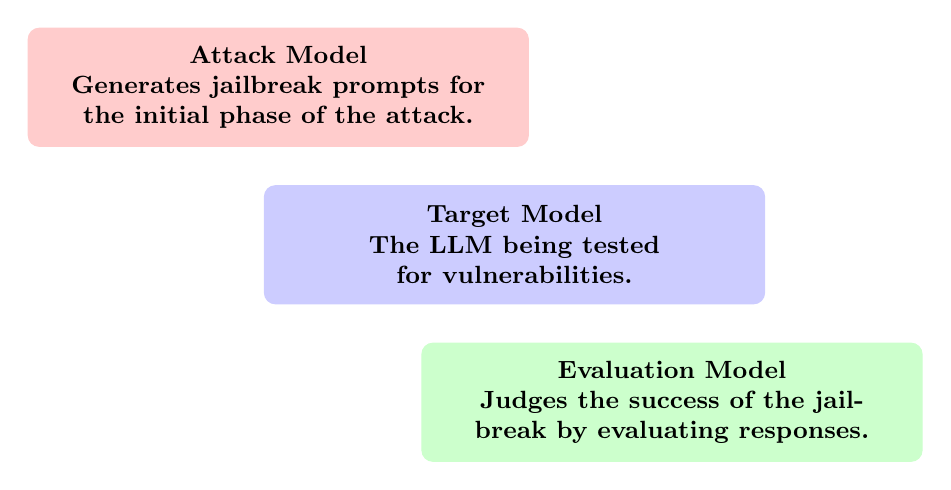
\begin{tikzpicture}[ 
        node distance=1cm, 
        every node/.style={
            rectangle, draw, 
            rounded corners, 
            minimum width=6cm, minimum height=1.5cm, 
            align=center, text centered, 
            font=\bfseries\small, inner sep=5pt
        }
    ]
        % Attack Model Node
        \node[fill=red!20, draw=red!20, text width=6cm, anchor=center] (attack_model) at (5,2) {
            \textbf{Attack Model} \\ 
            Generates jailbreak prompts for the initial phase of the attack.
        };\pause
        % Target Model Node
        \node[fill=blue!20, draw=blue!20, text width=6cm, anchor=center] (target_model) at (8,0) {
            \textbf{Target Model} \\ 
            The LLM being tested for vulnerabilities.
        };\pause
        % Evaluation Model Node
        \node[fill=green!20, draw=green!20, text width=6cm, anchor=center] (evaluation_model) at (10,-2) {
            \textbf{Evaluation Model} \\ 
            Judges the success of the jailbreak by evaluating responses.
        };
    \end{tikzpicture}
\end{frame}


% \begin{frame}{Steps To Conduct A Jailbreak Attack}
%     \begin{enumerate}
%         \item Preparation 
%         \item Selector
%         \item Mutator
%         \item Constraint
%         \item Evaluator
%         \item Report
%     \end{enumerate}
% \end{frame}

% \begin{frame}{Preparation}
%     Preparation involves setting up the jailbreak attack by:
%     \begin{itemize}
%         \item Defining the \textbf{queries}.
%         \item Choosing the \textbf{seeds}.
%         \item Selecting the \textbf{models}.
%         \item Configuring \textbf{hyperparameters}.
%     \end{itemize}
% \end{frame}

% \begin{frame}{Understanding the Key Terms}
%     What are \textbf{queries}, \textbf{seeds}, \textbf{models}, and \textbf{hyperparameters}? \pause
%     Let's break it down with an example.
% \end{frame}

% \begin{frame}{Preparation: Game Metaphor}
%     Think of preparing for a jailbreak attack as setting up a game:
%     \begin{itemize}
%         \item \textbf{Queries}: The game challenges (e.g., asking "How to make a bomb?").
%     \end{itemize}
% \end{frame}

% \begin{frame}{Preparation: Game Metaphor (continued)}
%     \begin{itemize}
%         \item \textbf{Seeds}: The mission briefings, starting points for the attack.
%     \end{itemize}
% \end{frame}

% \begin{frame}{Preparation: Game Metaphor (continued)}
%     \begin{itemize}
%         \item \textbf{Seeds}: The mission briefings, starting points for the attack.
%         \item \textbf{Models}: The game characters (LLMs) you're trying to defeat.
%         \item \textbf{Adjusting Hyperparameters}: Setting the difficulty level of the game.
%     \end{itemize}
% \end{frame}

% \begin{frame}{Selector}
%     The \textbf{Selector} picks the best input (weapon) for the attack, maximizing the chances of success. \pause
%     \begin{itemize}
%         \item Example: \textbf{EXP3SelectPolicy} uses a smart strategy to choose the best weapons based on past success.
%     \end{itemize}
% \end{frame}

% \begin{frame}{Mutator}
%     The \textbf{Mutator} upgrades your weapon to improve its effectiveness. \pause
%     \begin{itemize}
%         \item Example: A \textbf{Translation Mutator} turns the input (weapon) into a different language to bypass detection.
%     \end{itemize}
% \end{frame}

% \begin{frame}{Constraint}
%     \textbf{Constraint} a trap detector, ensuring your attack remains focused and valid. \pause
%     \begin{itemize}
%         \item Example: \textbf{DeleteOffTopic} removes any input that is off-topic.
%     \end{itemize}
% \end{frame}

% \begin{frame}{Evaluator}
%     The \textbf{Evaluator} checks whether you won the game by assessing the success of the attack. \pause
%     \begin{itemize}
%         \item Example: \textbf{ClassificationJudge} a judge who decides if the challenge (attack) was successful.
%     \end{itemize}
% \end{frame}

% \begin{frame}{Report}
%     Generates a detailed analysis of the jailbreak attack:
%     \begin{itemize}
%         \item Success rate
%         \item Attack details
%         \item Perplexity of responses
%         \item Insights into the effectiveness of the attack
%     \end{itemize}
% \end{frame}


% \section{Usage}
% \begin{frame}{EasyJailbreak: Simplified Model Security Checks}
%     \begin{itemize}
%         \item \textbf{Usage:} EasyJailbreak simplifies security testing for LLMs with a few lines of Python code, enabling users to analyze models using methods.
%         \item \textbf{Models:} 
%         \begin{itemize}
%             \item \textbf{Attack Model:} Generates jailbreak prompts for the initial phase of the attack.
%             \item \textbf{Target Model:} The LLM being tested for vulnerabilities.
%             \item \textbf{Evaluation Model:} Judges the success of the jailbreak by evaluating responses.
%         \end{itemize}
%     \end{itemize}
% \end{frame}



%% TURJO PART HERE

% TURJO Preambles

\setbeamercolor{structure}{fg=myred} % Color of text elements
\setbeamercolor{alerted text}{fg=red} % Color of alerted text (e.g., \alert{})
\setbeamercolor{block title}{bg=myred,fg=white} % Color of block titles
\setbeamercolor{block body}{bg=lightgray} % Color of block body
\setbeamercolor{block title alerted}{bg=myred,fg=white} % Color of block titles
\setbeamercolor{block body alerted}{bg=lightgray} % Color of block body
\setbeamercolor{itemize item}{fg=myred} % Color of itemize bullets
\setbeamercolor{itemize subitem}{fg=myred} % Color of sub-itemize bullets
\setbeamercolor{enumerate item}{fg=myred} % Color of enumerate bullets
\setbeamercolor{enumerate subitem}{fg=myred} % Color of sub-enumerate bullets
\setbeamercolor{title}{fg=myred} % Color of title
\setbeamercolor{author}{fg=black} % Color of author
\setbeamercolor{date}{fg=black} % Color of date


\section{LLM Benchmarking}

\definecolor{myGreenTextColor}{rgb}{0.078, 0.69, 0.129}
\begin{frame}{Why is Benchmarking Important?}
    \begin{tikzpicture}[node distance=1.5cm and 1cm]
        
        % Define styles for blocks
        \tikzstyle{security} = [rectangle, fill=blue!10, 
                text width=8cm, rounded corners, 
                text centered, minimum height=1cm,
                minimum width = \textwidth,align=left
                ]
        \tikzstyle{model} = [rectangle, fill=red!10, 
                text width=8cm, rounded corners, 
                text centered, minimum height=1cm,
                minimum width = \textwidth,align=left
                ]
        \tikzstyle{effectiveness} = [rectangle, fill=orange!10, 
                text width=8cm, rounded corners, 
                text centered, minimum height=1cm,
                minimum width = \textwidth,align=left
                ]
        \tikzstyle{improvement} = [rectangle, fill=cyan!10, 
                text width=8cm, rounded corners, 
                text centered, minimum height=1cm,
                minimum width = \textwidth,align=left
                ]
        % Security Block
        \onslide<1->{
            \node[security] (security) at (0, 0) {%
                \begin{columns}
                    \column{0.1\textwidth}
                        \includegraphics[width=1cm]{stickers/security.png}
                    \column{0.9\textwidth}
                        \textbf{Security:} Helps identify vulnerabilities in LLMs.
                \end{columns}
            };
        }

        % Model Block
        \onslide<2->{
            \node[model] (model) [below of=security] {%
                \begin{columns}
                    \column{0.1\textwidth}
                        \includegraphics[width=1cm]{stickers/res.png}
                    \column{0.9\textwidth}
                        \textbf{Resistant:} Measures how resistant models are to jailbreak attacks.
                \end{columns}
            };
        }

        % Effectiveness Block
        \onslide<3->{
            \node[effectiveness] (effectiveness) [below of=model] {%
                \begin{columns}
                    \column{0.1\textwidth}
                        \includegraphics[width=1cm]{stickers/effectiveness.png}
                    \column{0.9\textwidth}
                        \textbf{Effectiveness:} Shows which methods work best to bypass models.
                \end{columns}
            };
        }

        % Improvement Block
        \onslide<4->{
            \node[improvement] (improvement) [below of=effectiveness] {%
                \begin{columns}
                    \column{0.1\textwidth}
                        \includegraphics[width=1cm]{stickers/improvement.png}
                    \column{0.9\textwidth}
                        \textbf{Improvement:} Provides insights for strengthening LLM security.
                \end{columns}
            };
        }

    \end{tikzpicture}
\end{frame}



\begin{frame}
    \frametitle{
        \begin{tabular}{c@{\hspace{0.5cm}}c@{\hspace{0.3cm}}c@{\hspace{0.3cm}}c}
            \raisebox{0.1cm}{{Models Tested}} & 
            \includegraphics[width=0.6cm]{stickers/gpt.png} & 
            \includegraphics[width=0.6cm]{stickers/Llama.png} & 
            \includegraphics[width=0.6cm]{stickers/Qwen.png}
        \end{tabular}
    }

    \begin{block}{LLM Models Used}
        
        \begin{tikzpicture}[node distance=.5cm]
            
            \tikzstyle{arrow} = [thick,->,>=stealth]
            
            % Open-source Models
            \onslide<2->{
                \node at ([xshift=1cm, yshift=-1cm]current page.north west) 
                {\includegraphics[width=0.8cm]{stickers/opensrc.png}};
            \node[anchor=west] at ([xshift=2cm, yshift=-1cm]current page.north west) {\textcolor{red}{Open-source Models}: LLaMA2, Vicuna, ChatGLM3, Qwen-7B};
        }
        
        % Closed-source Models
        \onslide<3->{
            \node at ([xshift=1cm, yshift=-2cm]current page.north west) 
            {\includegraphics[width=0.8cm]{stickers/colsesrc.png}};
            \node[anchor=west] at ([xshift=2cm, yshift=-2cm]current page.north west) {\textcolor{red}{Closed-source Models}: GPT-4, GPT-3.5-Turbo};
        }

        
    \end{tikzpicture}
    \end{block}
\end{frame}

\begin{frame}{An Important Question}
    \begin{columns}
        \column{0.3\textwidth}
        \includegraphics[width=3cm]{stickers/brainStorming.png}
        \column{0.65\textwidth}
        \begin{block}{Which one is better}
            \onslide<2->{Does an open-source model like LLaMA2 perform better than a closed-source model like GPT-4?}
        \end{block}
    \end{columns}
\end{frame}

\begin{frame}{Attack Method: Human Design}
    \begin{figure}
        \centering
        \resizebox{\textwidth}{!}{%
        \begin{tikzpicture}[node distance=1.5cm and 1cm]
            
            % Style for central node (attack method)
            \tikzstyle{method} = [rectangle, fill=blue!10, 
            text centered, rounded corners, minimum height=1cm, minimum width=3cm]
            
            % Style for example nodes (examples of the attack methods)
            \tikzstyle{example} = [rectangle, fill=red!10, 
            text centered, minimum height=1cm, minimum width=2.5cm]

            % Attack Method Node: Human Design
            \onslide<1->{
                \node[method] (human) {
                    \raisebox{-0.2cm}{\includegraphics[width=0.5cm]{stickers/coding.png}} \hspace{0.2cm} \textbf{Human Design}
                };
            }

            % Example Node for JailBroken with Icon Inside Text
            \onslide<2->{ % Show JailBroken on Slide 2
                \node[example, below left=of human, align=left, text width=3.5cm, xshift=1cm] (jailbroken) {
                    \faLockOpen\ \textbf{JailBroken:} Tricks the AI by acting like it's in a pretend scenario to make it ignore safety rules.
                };
                \draw[->, thick] (human) -- (jailbroken);
            }

            % Example Node for DeepInception with Icon Inside Text
            \onslide<3->{ % Show DeepInception on Slide 3
                \node[example, below right=of human, align=left, text width=3.5cm, xshift=-1cm] (deepinception) {
                    \faBrain\ \textbf{DeepInception:} Confuses the AI by sneaking tricky instructions into its context.
                };
                \draw[->, thick] (human) -- (deepinception);
            }

        \end{tikzpicture}
        }
    \end{figure}
\end{frame}





% Frame 2: Long-tail Encoding
\begin{frame}{Attack Method: Long-tail Encoding}
    \begin{figure}
        \centering
        \resizebox{\textwidth}{!}{%
        \begin{tikzpicture}[node distance=1.5cm and 1cm]

        % Style for central node (attack method)
        \tikzstyle{method} = [rectangle, fill=blue!10, 
                            text centered, rounded corners, minimum height=1cm, minimum width=3cm]

        % Style for example nodes (examples of the attack methods)
        \tikzstyle{example} = [rectangle, fill=red!10, 
                            text centered, minimum height=1cm, minimum width=2.5cm]

        % Attack Method Node: Long-tail Encoding
        \onslide<1->{
            \node[method] (longtail) {
                \raisebox{-0.2cm}{\includegraphics[width=0.5cm]{stickers/encode.png}} \hspace{0.2cm} \textbf{Long-tail Encoding}
            };
        }

        % Example Node for Cipher with Icon Inside Text
        \onslide<2->{\node[example, below left=of longtail, align=left, text width=3.5cm,xshift=1cm] (cipher) {
            \faKey\ \textbf{Cipher:} Hides the message by turning it into a code (like Morse or Base64) that the AI doesn't recognize as harmful.
            };
            \draw[->, thick] (longtail) -- (cipher);}

        % Example Node for MultiLingual with Icon Inside Text
        \onslide<3->{\node[example, below right=of longtail, align=left, text width=3.5cm,xshift=-1cm] (multilingual) {
            \faLanguage\ \textbf{MultiLingual:} Uses uncommon languages that the AI isn't fully trained on to slip past its defenses.
        };

        % Arrows from central node to examples
        \draw[->, thick] (longtail) -- (multilingual);}

        \end{tikzpicture}
    }
    \end{figure}
\end{frame}





% Frame 3: Prompt Optimization
\begin{frame}{Attack Method: Prompt Optimization}
    \begin{figure}
        \centering
        \resizebox{\textwidth}{!}{%
    \begin{tikzpicture}[node distance=1.5cm and 1cm]

    % Style for central node (attack method)
    \tikzstyle{method} = [rectangle, fill=blue!10, 
                          text centered, rounded corners, minimum height=1cm, minimum width=3cm]

    % Style for example nodes (examples of the attack methods)
    \tikzstyle{example} = [rectangle, fill=red!10, 
                           text centered, minimum height=1cm, minimum width=2.5cm]

    % Attack Method Node: Prompt Optimization
    \onslide<1->{
        \node[method] (prompt) {
            \raisebox{-0.2cm}{\includegraphics[width=0.5cm]{stickers/speed-radar.png}} \hspace{0.2cm} \textbf{Prompt Optimization}
        };
    }


    % Example Node for GPTFUZZER with Icon
    \onslide<2->{\node[example, below left=of prompt, align=left, text width=3.5cm] (gptfuzzer) {
        \includegraphics[width=0.5cm]{stickers/GPTFUZZER.png}\hspace{0.2cm}\textbf{GPTFUZZER:} 
        Tries out different versions of the same question to find one that the AI will answer incorrectly.
    };
    \draw[->, thick] (prompt) -- (gptfuzzer);}

    % Example Node for PAIR with Icon
    \onslide<3->{\node[example, below=of prompt, align=left, text width=3.5cm] (pair) {
        \includegraphics[width=0.5cm]{stickers/robot.png}\hspace{0.2cm}\textbf{PAIR:} 
        Improves questions step-by-step based on how the AI responds, making them more likely to bypass safety.
    };
    \draw[->, thick] (prompt) -- (pair);}

    % Example Node for AutoDAN with Icon
    \onslide<4->{\node[example, below right=of prompt, align=left, text width=3.5cm] (autodan) {
        \includegraphics[width=0.5cm]{stickers/Robot-Hand-PNG-Photos.png}\hspace{0.2cm}\textbf{AutoDAN:} 
        Uses trial and error to keep changing the question until the AI gives the desired response.
    };
    \draw[->, thick] (prompt) -- (autodan);}

    % Arrows from central node to examples

    \end{tikzpicture}
    }
    \end{figure}
\end{frame}

\begin{frame}{Benchmarking Results}
    \centering
    \begin{tikzpicture}

        % Title
        \node[anchor=north, font=\large\bfseries] at (6, 5) {Key Findings};

        % Avg. Breach Progress Bar
        \onslide<1->{ % Show Avg. Breach on Slide 1
            \node[anchor=west, font=\bfseries] at (0, 3.5) {Avg. Breach:};
            \draw[black] (4, 3.4) rectangle (10, 3.7);
            \node[anchor=west, font=\bfseries] at (10.5, 3.6) {\textcolor{blue!60}{63\%}};
            \fill[blue!60] (4, 3.4) rectangle (7.78, 3.7);
        }

        % GPT-3.5-Turbo Progress Bar
        \onslide<2->{ % Show GPT-3.5-Turbo on Slide 2
            \node[anchor=west, font=\bfseries] at (0, 3) {GPT-3.5-Turbo:};
            \draw[black] (4, 2.9) rectangle (10, 3.2);
            \node[anchor=west, font=\bfseries] at (10.5, 3.1) {\textcolor{red!60}{57\%}};
            \fill[red!60] (4, 2.9) rectangle (7.42, 3.2);
        }

        % GPT-4 Progress Bar
        \onslide<3->{ % Show GPT-4 on Slide 3
            \node[anchor=west, font=\bfseries] at (0, 2.5) {GPT-4:};
            \draw[black] (4, 2.4) rectangle (10, 2.7);
            \node[anchor=west, font=\bfseries] at (10.5, 2.6) {\textcolor{myGreenTextColor!60}{33\%}};
            \fill[myGreenTextColor!60] (4, 2.4) rectangle (5.89, 2.7);
        }

        % Vicuna-13B Progress Bar
        \onslide<4->{ % Show Vicuna-13B on Slide 4
            \node[anchor=west, font=\bfseries] at (0, 2) {Vicuna-13B:};
            \draw[black] (4, 1.9) rectangle (10, 2.2);
            \node[anchor=west, font=\bfseries] at (10.5, 2.1) {\textcolor{orange!60}{83\%}};
            \fill[orange!60] (4, 1.9) rectangle (8.98, 2.2);
        }

        % Comment or Note
        \onslide<5->{ % Show Note on Slide 5
            \node[anchor=west, font=\large\itshape, text width=12cm] at (0, 1) 
                {Note: Larger models are not inherently more secure. Breach percentages indicate vulnerability.};
        }
    \end{tikzpicture}
\end{frame}


\begin{frame}{Performance Metrics: ASR}
    \begin{figure}
        \centering
        \resizebox{\textwidth}{!}{%
        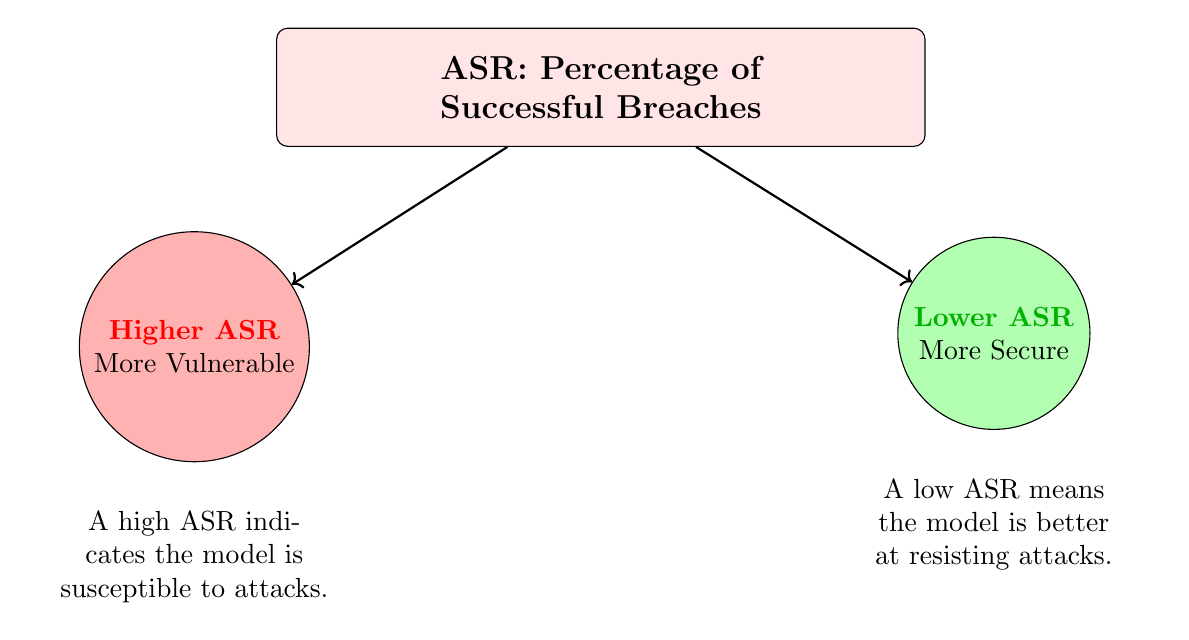
\begin{tikzpicture}[node distance=1.5cm and 2cm]

            % Main Title Node
            \onslide<1->{ % Show ASR Title on Slide 1
                \node[draw, rectangle, fill=red!10, text width=8cm, rounded corners, text centered, 
                minimum height=1.5cm, font=\large\bfseries] (asr) 
                {ASR: \textbf{Percentage of Successful Breaches}};
            }

            % Vulnerability Node
            \onslide<2->{ % Show Vulnerability Node on Slide 2
                \node[draw, circle, fill=red!30, below left=of asr, minimum size=2cm, text centered, 
                align=center, xshift=2cm] (vulnerable) {\textbf{\textcolor{red}{Higher ASR}} \\ More Vulnerable};
                \draw[->, thick] (asr) -- (vulnerable);
            }

            % Vulnerability Note
            \onslide<3->{ % Show Note for Higher ASR on Slide 3
                \node[below=0.5cm of vulnerable, text width=4cm, text centered] 
                (note1) {A high ASR indicates the model is susceptible to attacks.};
            }

            % Security Node
            \onslide<4->{ % Show Security Node on Slide 4
                \node[draw, circle, fill=green!30, below right=of asr, minimum size=2cm, text centered, 
                align=center, xshift=-2cm] (secure) {\textbf{\textcolor{green!70!black}{Lower ASR}} \\ More Secure};
                \draw[->, thick] (asr) -- (secure);
            }

            % Security Note
            \onslide<5->{ % Show Note for Lower ASR on Slide 5
                \node[below=0.5cm of secure, text width=4cm, text centered] 
                (note2) {A low ASR means the model is better at resisting attacks.};
            }

        \end{tikzpicture}
        }
    \end{figure}
\end{frame}


\begin{frame}{Performance Metrics: Efficiency}
    \begin{figure}
        \centering
        \resizebox{\textwidth}{!}{%
        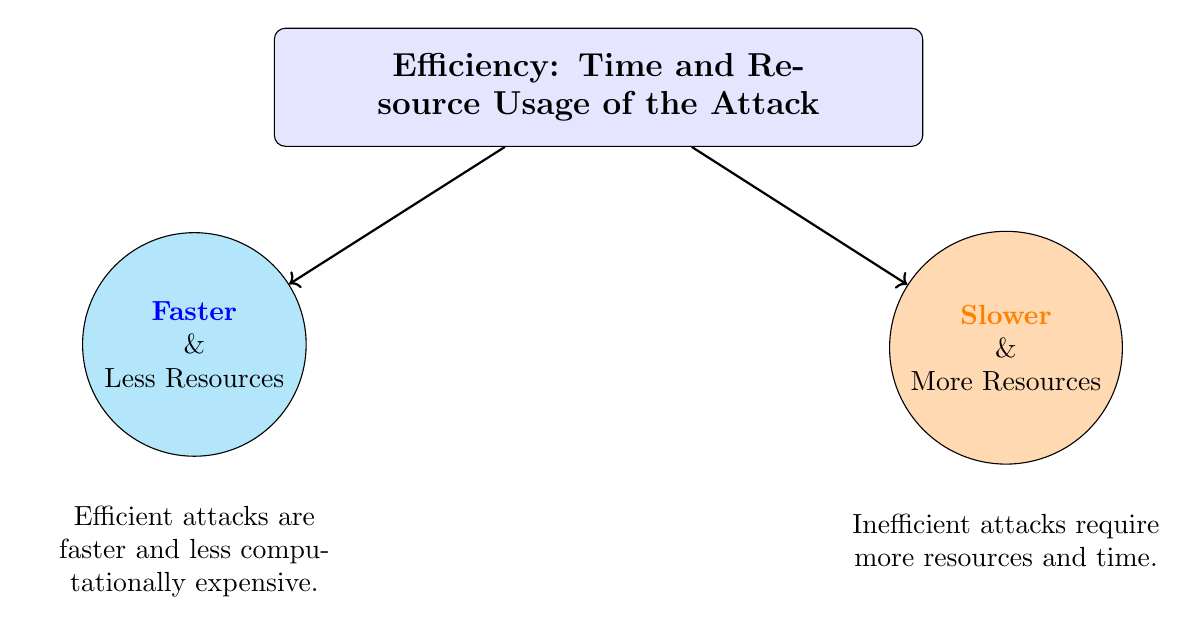
\begin{tikzpicture}[node distance=1.5cm and 2cm]

            % Main Title Node
            \onslide<1->{ % Show Efficiency Title on Slide 1
                \node[draw, rectangle, fill=blue!10, text width=8cm, rounded corners, text centered, 
                minimum height=1.5cm, font=\large\bfseries] (efficiency) 
                {Efficiency: \textbf{Time and Resource Usage of the Attack}};
            }

            % Faster Node
            \onslide<2->{ % Show Faster Node on Slide 2
                \node[draw, circle, fill=cyan!30, below left=of efficiency, minimum size=2cm, text centered, 
                align=center, xshift=2cm] (faster) {\textbf{\textcolor{blue}{Faster}} \\ \& \\ Less Resources};
                \draw[->, thick] (efficiency) -- (faster);
            }

            % Faster Node Note
            \onslide<3->{ % Show Note for Faster on Slide 3
                \node[below=0.5cm of faster, text width=4cm, text centered] 
                (note1) {Efficient attacks are faster and less computationally expensive.};
            }

            % Slower Node
            \onslide<4->{ % Show Slower Node on Slide 4
                \node[draw, circle, fill=orange!30, below right=of efficiency, minimum size=2cm, text centered, 
                align=center, xshift=-2cm] (slower) {\textbf{\textcolor{orange}{Slower}} \\ \& \\ More Resources};
                \draw[->, thick] (efficiency) -- (slower);
            }

            % Slower Node Note
            \onslide<5->{ % Show Note for Slower on Slide 5
                \node[below=0.5cm of slower, text width=4cm, text centered] 
                (note2) {Inefficient attacks require more resources and time.};
            }

        \end{tikzpicture}
        }
    \end{figure}
\end{frame}



\begin{frame}{ASR Comparison (Llama2-7B vs Llama2-13B)}
    \begin{columns}
        \column{0.6\textwidth}
        \begin{figure}[ht]
            \centering
            \includegraphics[width=\linewidth]{pic/Llama_comparison.pdf}
            \caption{ASR of Llama models}
            \label{fig:asr_plot_Llama}
        \end{figure}
        \column{0.35\textwidth}\pause
            \begin{block}{Summary}
            \begin{itemize}
                \item \textcolor{red}{Llama2-13B:       \textbf{37\%}},  \textcolor{myGreenTextColor}{Llama2-7B: \textbf{31\%}}.\pause
                \item Bigger models $\neq$ better security.\pause
                \item Cipher, Prompt Optimization work better for \textcolor{myGreenTextColor}{Llama2-13B}.
            \end{itemize}
        \end{block}        
    \end{columns}
\end{frame}
\begin{frame}{ASR Comparison (GPT-3.5-turbo vs GPT-4-0613)}
    \begin{columns}
        \column{0.65\textwidth}
        \begin{figure}[ht]
            \centering
            \includegraphics[width=\linewidth]{pic/GPT_comparison.pdf}
            \caption{ASR of GPT Models}
            \label{fig:asr_plot_gpt}
        \end{figure}
        \column{0.25\textwidth}\pause
            This shows that larger models are not always better as Llama-7B (\textcolor{myGreenTextColor}{31\%}) has better ASR than GPT-4-0613 (\textcolor{red}{33\%})
    \end{columns}
\end{frame}
\begin{frame}{Efficiency Comparison (Llama2-7B vs Llama2-13B)}
    \begin{columns}
        \column{0.6\textwidth}
        \begin{figure}[ht]
            \centering
            \includegraphics[width=\linewidth]{pic/comparison_plot_2.pdf}
            \caption{Efficiency Comparison (Llama)}
            \label{fig:asr_plot_2}
        \end{figure}
        \column{0.35\textwidth}\pause
            \begin{block}{Summary}
            \begin{itemize}
                \item \textcolor{red}{Llama2-13B} takes more time.\pause
                \item Prompt Optimization: Slow but better results.\pause
                \item Cipher: Efficient and effective.
            \end{itemize}
        \end{block}
            
    \end{columns}
\end{frame}

\begin{frame}{Time-Resource Trade-offs (Llama)}
    \begin{figure}[h]
        \centering
        \includegraphics[width=\textwidth]{pic/accuracy_and_time_consumption_chart.pdf}
        \caption{Time vs. resource efficiency for different attacks.}
        \label{fig:time_res_trade}
    \end{figure}
\end{frame}

\begin{frame}{Trade-Off: Model Size vs Efficiency}
    \begin{figure}
        \centering
        \resizebox{\textwidth}{!}{%
        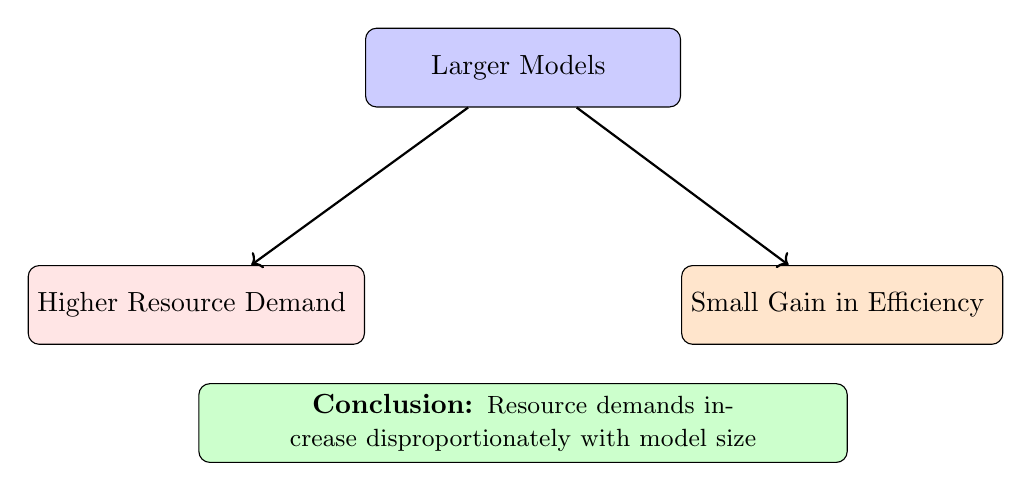
\begin{tikzpicture}[
            node distance=2cm and 2cm,
            every node/.style={align=center},
            box/.style={draw, rectangle, rounded corners, minimum width=4cm, minimum height=1cm, text centered, fill=blue!10},
            arrow/.style={->, thick}
        ]

            % Node: Larger Models
            \onslide<1->{ % Show Larger Models on Slide 1
                \node[box, fill=blue!20] (largemodels) {Larger Models
                % \\ (e.g., Llama2-13B)
                };
            }

            % Node: Increased Resources
            \onslide<2->{ % Show Increased Resources on Slide 2
                \node[box, below left=of largemodels, fill=red!10, xshift=2cm] (resources) {Higher Resource Demand
                % \\ (Memory, Time, Compute)
                };
                \draw[arrow] (largemodels) -- (resources);
            }

            % Node: Marginal Gains
            \onslide<3->{ % Show Marginal Gains on Slide 3
                \node[box, below right=of largemodels, fill=orange!20, xshift=-2cm] (marginalgains) {Small Gain in Efficiency
                % \\ (Success Rate vs Time)
                };
                \draw[arrow] (largemodels) -- (marginalgains);
            }

            % Conclusion Node
            \onslide<4->{ % Show Conclusion on Slide 4
                \node[box, below=3.5cm of largemodels, fill=green!20, text width=8cm] (conclusion) {
                    \textbf{Conclusion:} \small{Resource demands increase disproportionately with model size
                    % , requiring careful trade-offs when deploying larger models.
                    }
                };
            }

        \end{tikzpicture}
        }
    \end{figure}
\end{frame}





\section{Conclusion}

\begin{frame}{Key Findings - Summary}
    \begin{tikzpicture}[node distance=1.5cm and 1cm]

        % Define styles for blocks
        \tikzstyle{vulnerability} = [rectangle, fill=blue!10, 
                text width=8cm, rounded corners, 
                text centered, minimum height=1cm,
                minimum width = \textwidth,align=left
                ]
        \tikzstyle{advancedmodels} = [rectangle, fill=red!10, 
                text width=8cm, rounded corners, 
                text centered, minimum height=1cm,
                minimum width = \textwidth,align=left
                ]
        \tikzstyle{opensource} = [rectangle, fill=orange!10, 
                text width=8cm, rounded corners, 
                text centered, minimum height=1cm,
                minimum width = \textwidth,align=left
                ]
        \tikzstyle{largermodels} = [rectangle, fill=cyan!10, 
                text width=8cm, rounded corners, 
                text centered, minimum height=1cm,
                minimum width = \textwidth,align=left
                ]

        % Vulnerability Block
        \onslide<1->{
            \node[vulnerability] (vulnerability) at (0, 0) {%
                \begin{columns}
                    \column{0.1\textwidth}
                        \includegraphics[width=1cm]{stickers/vulnerability.png}
                    \column{0.85\textwidth}
                        \textbf{Vulnerability:} All tested models exhibit vulnerabilities to jailbreak attacks.
                \end{columns}
            };
        }

        % Advanced Models Block
        \onslide<2->{
            \node[advancedmodels] (advancedmodels) [below of=vulnerability] }).
                \end{columns}
            };
        }

        % Open-Source Models Block
        \onslide<3->{
            \node[opensource] (opensource) [below of=advancedmodels] {%
                \begin{columns}
                    \column{0.1\textwidth}
                        \includegraphics[width=1cm]{stickers/opensrc.png}
                    \column{0.85\textwidth}
                        \textbf{Open-Source Models:} \textcolor{red}{\textbf{Vicuna}} have higher average breach probabilities.
                \end{columns}
            };
        }

        % Larger Models Block
        \onslide<4->{
            \node[largermodels] (largermodels) [below of=opensource] {%
                \begin{columns}
                    \column{0.1\textwidth}
                        \includegraphics[width=1cm]{stickers/large.png}
                    \column{0.85\textwidth}
                        \textbf{Larger Models:} Does not guarantee better security.
                \end{columns}
            };
        }

    \end{tikzpicture}
\end{frame}


\begin{frame}{Key Findings - Comparison}
    \begin{figure}
        \centering
        \resizebox{\textwidth}{!}{%
            \begin{tikzpicture}[
                node distance=1.5cm and 2cm,
                every node/.style={align=center}
            ]

                % Nodes for Open-Source and its Finding
                \onslide<1->{\node[draw, rectangle, fill=blue!10, rounded corners, minimum width=4cm, minimum height=1cm] 
                    (opensource) {Open-Source Models};}
                \onslide<2->{\node[draw, rectangle, fill=red!10, rounded corners, right=1.2cm of opensource, minimum width=0.6\textwidth, text width=0.6\textwidth] 
                    (opensourcefinding) {\textbf{Higher vulnerability} to attacks\\ Example: Vicuna models show higher breach rates.};}

                % Nodes for Closed-Source and its Finding
                \onslide<1->{\node[draw, rectangle, fill=blue!10, rounded corners, below=1.5cm of opensource, minimum width=4cm, minimum height=1cm] 
                    (closedsource) {Closed-Source Models};}
                \onslide<3->{\node[draw, rectangle, fill=red!10, rounded corners, right=1.2cm of closedsource, minimum width=0.6\textwidth, text width=0.6\textwidth] 
                    (closedsourcefinding) {\textbf{Lower average breach rates}\\ Example: GPT-4 is more resistant to attacks.};}

                % Conclusion Node (Same Width as Finding Nodes)
                \onslide<4->{\node[draw, rectangle, fill=green!20, rounded corners, below=2cm of closedsource, minimum width=0.8\textwidth, text width=0.8\textwidth, font=\bfseries,anchor=west,xshift=-0.5cm]
                    (conclusion) {\textbf{Conclusion:}\\ \textcolor{myGreenTextColor}{\textbf{Closed-source}} models generally provide \textbf{better resistance} to jailbreaks.};}

            \end{tikzpicture}
        }
    \end{figure}
\end{frame}


\begin{frame}{Implications and Future Directions}
    \setbeamercolor{block title}{bg=red,fg=white}
    \setbeamercolor{block body}{bg=red!10,fg=black}

    \begin{block}{Implications:}
        \begin{itemize}
            \item \small{Stronger defenses.} \pause
            \item \small{Continuous security validation.} \pause
        \end{itemize}
    \end{block}

    \setbeamercolor{block title}{bg=myGreenTextColor,fg=white}
    \setbeamercolor{block body}{bg=myGreenTextColor!10,fg=black}

    \definecolor{newGreen}{rgb}{0.169, 0.388, 0.145}

    \setbeamercolor{itemize item}{fg=newGreen} % Color of itemize bullets
    \setbeamercolor{itemize subitem}{fg=myred} % Color of sub-itemize bullets

    \begin{block}{Future Work:}
        \begin{itemize}
            \item \small{Develop modular defenses for prompt attacks.} \pause
            \item \small{Test larger models (e.g., LLaMA2-70B).} \pause
            \item \small{Enhance EasyJailbreak to counter new threats.}
        \end{itemize}
    \end{block}
\end{frame}

\begin{frame}[t]{Thank You!}
    
    \begin{tikzpicture}[remember picture, overlay]

        % Person Image in the Center
        \node[anchor=center] (person) at (current page.center) {
            \includegraphics[width=4cm]{stickers/thanksPerson.png}
        };

        % Bubble Image on Top Left of the Person
        \node[anchor=south west] at ([xshift=-0.5cm, yshift=-1.5cm]person.north east) {
            \includegraphics[width=2.5cm]{stickers/thanks.png}
        };

    \end{tikzpicture}

    % Optional Text Below Person
    \vspace{5cm}
    \centering
    {\huge Thank You for Your Attention!}
\end{frame}



\end{document}